\documentclass[uplatex,twocolumn,dvipdfmx,10pt]{jsarticle}
\usepackage[top=22mm,bottom=22mm,left=19mm,right=19mm]{geometry}
\renewcommand{\baselinestretch}{0.9}
\setlength{\columnsep}{10mm}
\usepackage[T1]{fontenc}
\usepackage{txfonts}
\usepackage[expert,deluxe]{otf}
\usepackage[dvipdfmx,hiresbb]{graphicx}
\usepackage[dvipdfmx]{hyperref}
\usepackage{pxjahyper}
\usepackage{secdot}
\makeatletter
\g@addto@macro{\UrlBreaks}{\UrlOrds}
\makeatother




%タイトルと学生番号,氏名だけ編集する.
\title{\vspace{-5mm}\fontsize{14pt}{0pt}\selectfont 動画投稿サービスにおける有料コメントシステムの利用に関する調査\\
{\normalsize Survey on the use of paid commenting systems in video posting services}}
\author{\normalsize マネジメント工学専攻修士課程 矢吹研究室 1991007 島田光馬}
\date{}
\pagestyle{empty}
\begin{document}
\maketitle


\section{序論}

動画閲覧サイトでは,ビデオ内に広告を表示するIn-Video広告と呼ばれる提示形式が使用されている.In-Video広告は動画を視聴する妨げとなるため,不快に感じるユーザがいる\cite{01}.
そのため,動画サイトの一つであるYouTubeでは広告はスキップされることがある.
広告がスキップされると,配信者が広告費収入を得られなくなる.配信者にとっては,配信者が広告収入を得るための審査が厳しかったり,広告が掲載されなくなる基準が不透明であるという問題もある.そこで,広告ではなく,視聴者から直接対価を受け取れるしくみが広まってきている.YouTubeでは,そのしくみはスーパーチャット(以下,スパチャという)である.

YouTubeは,主にコミュニケーションツールとして使用される\cite{02}.
ライブ配信中に視聴者とコミュニケーションが取れることがYouTubeの魅力である.中でも,Vtuberに投資する人が多く存在する.
Vtuberとは,VirtualYouTuberの略で,コンピュータグラフィックスを用いて動画投稿・配信を行う人である.

本研究では,YouTubeで活動するライブ配信Vtuberを対象にし,ライブ配信のコメントとスパチャを収集し調査する.


\section{目的}

ライブ配信サービスにおける投げ銭システムを収集するためのツールを開発し,それを用いてコメントに比例して投げ銭が多いか調査する.

\section{手法}

本研究は以下の3段階で行う.
\begin{enumerate}
 \item YouTubeライブ配信のアーカイブからコメントとスパチャを取り出すためのツールを開発する.
 \item ライブ配信のチャットログからスパチャとコメントを集計する.
 \item コメントと時間,スパチャをヒストグラムで表す.
\end{enumerate}

\section{結果}

YouTubeは数か月おきにシステムアップデートが行われ,ブラウザも最新にする必要がある.そのため,selniumを使用しツールの開発した.ツールは配信した後に投稿される動画からチャットログを見つけ,コメントと時間,スパチャを取得する.
図1では,取得したスパチャの累計金額と時間を表している.
\begin{figure}[hbtp]
\begin{center} %センタリングする
%\includegraphics[width=図の幅,clip]{ファイル名}\label{参照用ラベル}
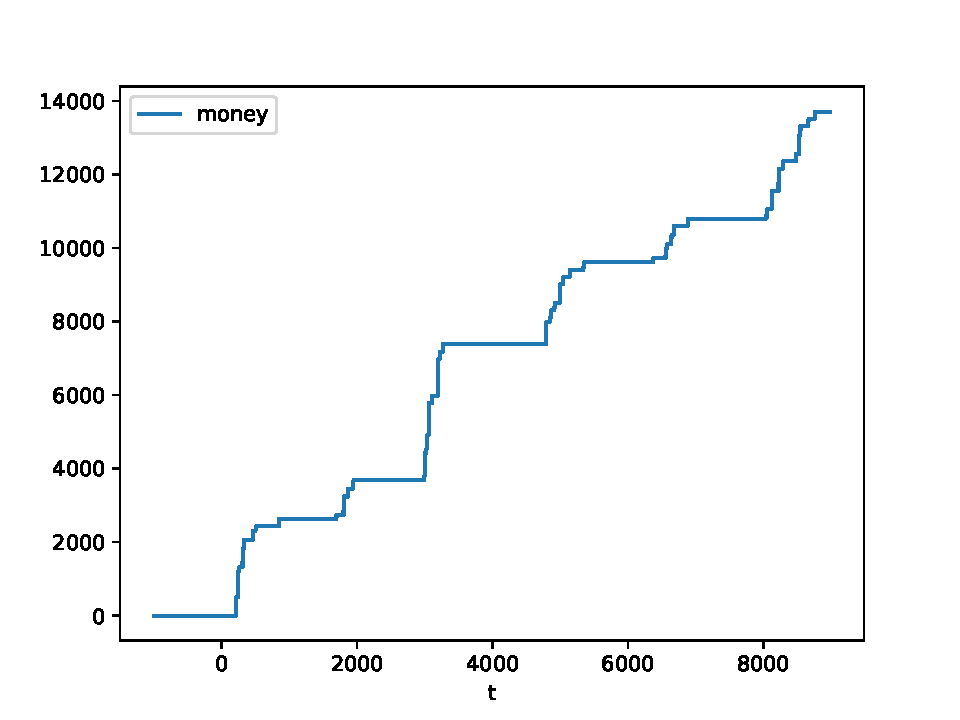
\includegraphics[width=7cm,clip]{livechatlog.pdf}
\caption{放送時間に対する累計金額}\label{time}
\end{center}
\end{figure}


\section{考察}
調査した結果,スパチャには,円やドル,ユーロなど様々なお金が存在し,多くが円で投げ銭をしていた.
配信を始めて中盤で一気に投げ銭が行われており,コメントでスパチャタイムと称されていたことも分かった.
各配信ごとに統計は変わっており,平均が2,000を超えることもある.


\section{結論}
ライブ配信サービスでよく使われている投げ銭について調査した.

YouTube APIでは制限がかかり使えず,投げ銭システムを収集するツールの開発を行った.
開発したシステムを使って投げ銭のログを取得し,基本的な統計量を調査した.大量の動画への投げ銭を解析し,投げ銭を受ける配信者の特徴や,投げ銭を投げる視聴者の特徴を調べることが今後の課題である.




\bibliographystyle{junsrt}
\bibliography{biblio}

\end{document}
